\documentclass[a4paper, 12pt]{ctexart}
\usepackage[UTF8]{ctex}
\usepackage{graphicx}
\usepackage{grffile}
\usepackage{longtable}
\usepackage{wrapfig}
\usepackage{rotating}
\usepackage{amsmath}
\usepackage{mathrsfs}
\usepackage{amssymb} 
\usepackage{amsmath} 
\usepackage{amsthm}
\usepackage{xltxtra} 
\usepackage{mflogo,texnames}
\usepackage{indentfirst}
\usepackage[normalem]{ulem}
\usepackage{textcomp}
\usepackage{booktabs}
\usepackage[linktocpage,pdfstartview=FitH,colorlinks,
linkcolor=blue,anchorcolor=blue,
citecolor=blue,filecolor=blue,menucolor=blue,urlcolor=blue]{hyperref}
\usepackage{setspace,csquotes, enumitem,endnotes,fontspec, capt-of}
\doublespacing
\usepackage[margin=1in]{geometry}
\usepackage[notes, notetype=endonly, isbn=false, backend=biber]{biblatex-chicago}
\bibliography{shiff2016b}
\let\footnote=\endnote
\let\cite=\endnote
\let\footcite=\autocite
\setCJKmainfont{SimSun}
\CTEXsetup[format={\Large\bfseries}]{section}
\setlist[enumerate,itemize]{noitemsep,nolistsep,leftmargin=*}
\newtheorem*{theorem}{问题}%[section]

\author{张天骏 \\ 2024 Spring \\ 感谢王哲同学在题目解答方面提供的帮助}
\date{}
\title{泛函分析整理 \\ \large 刘培德《泛函分析基础:修订版》\\ 授课教师:朱朗峰}


\begin{document}
\maketitle


\newpage
\tableofcontents   


\newpage
\section{线性赋范空间}
\subsection{知识点速览}
\subsubsection{度量空间、赋范线性空间、内积空间}
\begin{enumerate}
    \item 度量$d$是关于空间两个点的距离的描述。基于这个概念我们可以定义一个点列关于某一个点的收敛:$d(x_n,x)\to 0$。这是我们后续大多数证明的终点。
    \item 范数是关于空间一个点的位置的描述,它给定了一个固定的参考点:原点。所以,若一个度量能诱导出范数,那它要满足一次齐次性和平移不变性。
    \item 内积,就是从$\mathbb{R}^n$中自然推广过来的。和$\mathbb{R}^n$中一样,若一个范数能诱导出内积,那么它要满足平行四边形公式(极化恒等式)。
    \item 极化恒等式:$(x,y)=\frac{1}{4}\left(||x+y||^2-||x-y||^2+i||x+iy||^2-i||x-iy||^2\right)$
    \begin{enumerate}
        \item $\text{Re}(x,y)=\frac{1}{4}\left(||x+y||^2-||x-y||^2\right)$
        \item $\text{Im}(x,y)=\frac{1}{4}\left(||x+iy||^2-||x-iy||^2\right)$
    \end{enumerate}
    \item 这一部分书上提供了丰富的例子,建议认真研读,感受。
\end{enumerate}
\subsubsection{$\mathbb{R}$上完备性定理在度量空间的推广}
\begin{enumerate}
    \item 首先,一般的度量空间中,柯西准则不一定成立。所以我们有必要首先定义完备性:满足柯西准则的空间,才能进一步操作。(所谓不完备的空间就是有"孔洞"的空间,有些点没有定义,但是附近有空间内的点列无限接近它)
    \item 有了完备性,我们可以推广"区间套定理"为"闭集套定理"
    \item 对于线性赋范空间,我们可以定义形式级数(点列的无穷和$\sum_{n=1}^\infty x_n$),进而定义它的可和性(可和,绝对可和)。
    进一步,我们可以推广"单调有界原理"为"绝对可和级数可和定理"
    \item 然而,在考虑紧集时,我们不再能够得出它与有界闭集的等价性。于是我们要重新定义紧性:基于有限覆盖这一本质。
    在度量空间中,紧性等价于无穷序列存在收敛子列,且极限点在集合内。在此有限覆盖定理和聚点定理(Bolzano-Weierstrass)被推广了。
    \item 接着上面的紧性,在一般的线性赋范空间中,有界集的性质也发生了畸变。于是我们又基于$\varepsilon-\text{网}$定义了更强的有界性:完全有界。
    在度量空间中,完全有界性等价于无穷序列存在柯西子列。完全有界的概念很有用,它给出了解构一个大集合的方法,通过$\varepsilon-\text{网}$。
    \item 在一般的度量空间,并未定义像$\mathbb{R}$一样的序关系,所以没有确界原理。
\end{enumerate}
\subsubsection{基于映射的同构、等价}

\subsubsection{稠密与纲:无限维完备线性赋范空间的维数是不可数的}
\begin{enumerate}
    \item 首先要了解稠密、无处稠密、纲的概念,这对于无限维的描述十分关键。
    \item 稠密性/无处稠密性的定义基于闭包,而闭包除去孤立点后,剩下聚点(内点+边界点),意味着“不可达的无限逼近”。
    \item 稠密性可以推广到任意一个闭集的子集:只要该子集的闭包是原集合,就说这个子集关于闭集稠密。由此来理解“无处稠密集”:关于哪个闭子集都不稠密;“全空间的稠密子集”:关于任意闭子集稠密。
    \item 至于纲,它基于集合的表示(第一纲集的可数并),将集合进行了分划,赋予"category"。基于纲,我们有著名的Baire纲定理:完备度量空间具有Baire性质:可数稠密子集的交仍稠密,这是第二纲集的充分条件。
    所以我们可以证明一个空间是第一纲的来证明它不完备:用这个思路可以证明无穷维完备赋范线性空间的维数是不可数的,不然就是一个第一纲集,矛盾。
    \item 接着,我们引入了可分集的概念:存在可数稠密子集。这是完全有界集的必要条件。同时,我们也可以定义可分空间。
\end{enumerate}
\subsubsection{走向无限维:无尽的量变最终引起质变}
\begin{enumerate}
    \item 首先要了解著名的Riesz引理,它表示线性赋范空间中,点到一个闭线性子空间的距离可以无限接近这个点的范数。
    \item 基于Riesz引理,我们可以刻画有限维空间的本质:有界闭集是紧集。而对于无限维空间,Riesz引理中的操作可以无限进行,
    从而构成一个点列没有收敛子列。特别地,有界闭集可以取闭单位球和闭单位球面。
\end{enumerate}
\subsection{习题(奇数题)}


\begin{theorem}
11:设$f \in \mathscr{L}^{\infty}(\Omega,\Sigma,\mu),\mu(\Omega)<\infty$,证明:
\\
(1) $||f||_\infty=\inf \{ C>0:\mu(|f|>C)=0 \}=\sup \{ C>0:\mu(|f|>C)>0 \}$
\\
(2) $||f||_\infty=\lim_{p \to \infty} ||f||_p$
\\
(3) 如果$||f||_\infty>0$,$||f||_\infty=\lim_{p \to \infty} \frac{||f||_{p+1}}{||f||_p}$
\end{theorem}

\begin{proof}
(1) 
$\exists c_{n}:\mu(A_{n}:\mid f\mid>c_{n}=0),  c_{n}>c_{0}:=\inf \{ C>0:\mu(|f|>C)=0 \},c_{n} \to c_{0}$
取$A=\bigcup_{n=1}^\infty:\mu(A)=0,c_{0}=\sup_{t\in U/A}\lvert f(t) \rvert\geq \lvert \lvert f \rvert \rvert_{\infty}$
记$E=\{ \lvert f \rvert>\lvert \lvert f \rvert \rvert_{\infty} \}$则按照范数定义:$\mu(E)=0$,所以$\lvert \lvert f \rvert \rvert_{\infty}\geq c_{0}$ 
所以$c_{0}=\lvert \lvert f \rvert \rvert_{\infty}$。
\\
而$\inf \{ C>0:\mu(|f|>C)=0 \}=\sup \{ C>0:\mu(|f|>C)>0 \}$是一个双重否定(零测集,正测集;下确界,上确界),所以二者等价
\\
(2)(3)略
\end{proof}

\begin{theorem}
17:设 $X$ 是 $[a,b]$ 上连续函数的全体,$1 \leq p < \infty$,
$$
\|x\|_{p}=\left(\int_{\alpha}^{\beta}|x(t)|^{p}\,\mathrm{d}t\right)^{\frac{1}{p}} \quad \forall x \in X.
$$
证明 $\|\cdot\|_{p}$ 是 $X$ 上的范数,但 $(X, \|\cdot\|_{p})$ 不是完备的。验证 $X$ 的完备化空间是 $L^{p}[\alpha,b]$.
\end{theorem}

\begin{proof}
先证明$\|\cdot\|_{p}$ 是 $X$ 上的范数:由于在该范数下,$C[a,b]\subset \mathscr{L}^p$。所以显然成立
\\
举反例证明不完备:考虑连续函数列$f_n(x)=\arctan(n(x-\frac{b-a}{2}))$,则$f(x):=\lim_{n\to \infty}f_n(x)=\mathbb{I}(x>\frac{b-a}{2})-\mathbb{I}(x<\frac{b-a}{2})$
很显然,$\lim_{n\to \infty}f_n(x)$不是连续函数,但是$f_n(x)\to f(X) \ \text{in norms}$,所以该赋范线性空间不完备。
\\
至于完备化的证明:因为连续函数可以逼近简单函数(Lusin Theorem),而简单函数全体在$\mathscr{L}^p$中稠密,所以$C[a,b]$是$\mathscr{L}^p$的一个稠密子集。
\end{proof}

\begin{theorem}
19:有可数Hamel基的线性赋范空间不是完备的。
\end{theorem}

\begin{proof}
设$\{x_n\}$是$X$的可数Hamel基,则$X=\bigcup_{n=1}^{\infty}\text{span}(x_n)$。但是在$X$中,每个$\text{span}(x_n)$都
不含内点,从而是无处稠密的。所以$X$是第一纲集,依Baire纲定理,完备度量空间的必要条件是第二纲的,所以$X$不完备。
\\(利用类似的方法还可以证明$[0,1]$区间是不可数的;无穷维Banach空间作为线性空间, 是不可数维的)
\end{proof}



\begin{theorem}
27:设 $l_{n}^\infty = \{x = (x_1, \cdots, x_n): x \in \mathbb{R}; \|x\| = \sup_{1 \leqslant i \leqslant n} |x_i|, \forall x \in l_{n}^\infty \}$。
定义线性算子 $T: l_{n}^\infty \to l_{n}^\infty$, $T$ 由 (1.3.7) 表达,证明当 $\sum_{j=1}^{n}|a_{ij}| < 1$ 时,算子方程 $Tx - x = y$ 有唯一解。
\end{theorem}

\begin{proof}
定义线性算子$V(x)=T(x)-y$,从而待证等价于证明$V$存在唯一的不动点。
因为$\lvert \lvert V(x_{1}-x_{2}) \rvert \rvert=\lvert \lvert T(x_{1}-x_{2}) \rvert \rvert\leq c\lvert \lvert x_{1}-x_{2} \rvert \rvert,0<c<1$;
又因为$l_{n}^\infty$是一个Banach空间,所以根据压缩映射定理,得证。
\end{proof}

\begin{theorem}
29:举例说明压缩映射定理中,如果映射条件放松到$d(Tx,Ty)<d(x,y)$时,结论不成立
\end{theorem}

\begin{proof}
举反例:$f(x)=2\pi+x-\arctan x$:$f$是Banach空间$\mathbb{R}\mapsto \mathbb{R}$的一个函数,
且$|f(x)-f(y)|=|(x-y)-(\arctan x-\arctan y)|<|x-y|$,因为$f'(x)=\frac{x^2}{1+x^2}<1$。
但是:方程$f(x)=x$即$\arctan x=2\pi$无解,所以不存在不动点。
\end{proof}

\begin{theorem}
31:对于度量空间$X$,下面两个命题等价:\\
(1) $X$ 是紧空间;\\
(2) 设 $\{F_{\lambda} : \lambda \in A\}$ 是 $X$ 中的任一闭集族,若 $F_{\lambda}$ 具有有限交性质(即其中任意有限个集合之交非空),则 $\bigcap_{\lambda \in A} F_{\lambda} \neq \varnothing$。
\end{theorem}
\begin{proof}
这其实就是紧集"有限覆盖"定义的逆否条件。验证这一点即可。
\end{proof}

\begin{theorem}
33:若函数序列$f_n(t)$在紧集$A$上等度连续且逐点收敛,则$f_n(t)$在A上一致收敛。
\end{theorem}

\begin{proof}
由于紧集$A$上的连续函数空间是Banach空间,所以只需要证明$\{f_n\}$是依范数柯西列即可。
依据等度连续性:对于任意$\varepsilon>0$,给定$\delta:|t-t'|<\delta \to |f(t)-f(t')|<\varepsilon_1$。
基于这个$\delta$,取紧集A的有限开覆盖$A=\bigcup_{i=1}^n A_i,\text{diam}(A_i)<\delta$。
对于每个$A_i$:取$\varepsilon_i>0$,给定一个点$t$:$\forall t'\in t,|f_m(t')-f_n(t')|\leq |f_n(t)-f_n(t')|+|f_m(t)-f_m(t')|+|f_m(t)-f_n(t)|$
只要$m,n>N(\varepsilon_i),|f_m(t')-f_n(t')|\leq 3\varepsilon_i:\underset{t'\in A_i}{\sup}|f_m(t')-f_n(t')|\leq 3\varepsilon_i$;
最后取$\varepsilon=\underset{n=1\cdots n}{\max}{\varepsilon_i}$,则$\underset{t'\in A}{\sup}|f_m(t')-f_n(t')|\leq 3\varepsilon$。得证。
\end{proof}

\section{空间$B(X,Y)$与$X^*$}
\subsection{知识点速览}
\subsubsection{有界线性算子$T$的几个等价条件}
\begin{enumerate}
    \item $T$在某一点连续
    \item $T$是连续算子(全局连续)
    \item $T$是有界算子
    \item $T$在某点有界邻域内有界:特别地,$T$在单位球中有界
    \item 存在$a>0:||Tx||<a||x||$ \\
    对于有界线性泛函$f$,还等价于下面两个条件:
    \item $N(f)$是闭集
    \item $N(f)$不是$X$的稠密子集
\end{enumerate}

\subsubsection{空间$B(X,Y),X^*$}
\begin{enumerate}
    \item 如果$Y$是Banach空间,则$B(X,Y)$是Banach空间;$X^*$是Banach空间:对于$B(X,Y)$中柯西列$\{T_n\}:\forall x\in X:\{f_n(x)\}$都是$Y$中的柯西点列;
    从而可以逐点定义极限$Tx$;此时$||T_n x - T_x||\leq\varepsilon||x||\forall x\in X:||T_n-T||\leq \varepsilon:T_n-T\in B(X,Y)$。
    所以$T=T_n-(T_n-T)\in B(X,Y)$。柯西列$\{T_n\}$的极限得以定义。
\end{enumerate}

\subsubsection{泛函四大定理}
\begin{enumerate}
    \item 共鸣定理:线性赋范空间 $X$ 到 线性赋范空间$Y$ 的有界线性算子族,如果在 $X$ 的一个第二纲集上点点有界,则一致有界: 
    $$\underset{ \lambda }{ \sup }|T_{\lambda}x|<\infty ,\forall x\in E(\text{第二纲集})\to \underset{ \lambda }{ \sup }\lvert \lvert T_{\lambda} \rvert \rvert= \underset{ \lambda }{ \sup } \underset{ x }{ \sup }\frac{\lvert T_{\lambda}x\lvert}{\lvert \lvert x \rvert \rvert}<\infty$$
    Banach-Steinhaus: Banach空间(保证极限存在) $X$ 到线性赋范空间 $Y$ 的一列有界线性算子如果点点收敛(自然点点有界),则可定义算子极限 $T:Tx=\lim_{ n \to \infty }T_{n}x$ 且 $$\lvert \lvert T \rvert \rvert\leq\underset{ n \to \infty }{ \varliminf }\lvert \lvert T_n \rvert \rvert$$
    \item 开算子定理:Banach 空间 $X$ 到线性赋范空间 $Y$ 的有界线性算子 $T$,如果像集$R(T)$是第二纲集,则 $T$ 是开算子且满射;Banach 空间 $X$ 到Banach 空间 $Y$ 上的有界线性算子 $T$ 是开算子。 \\
    逆算子定理:Banach 空间 $X$ 到线性赋范空间 $Y$ 的一一的有界线性算子 $T$,如果像集$R(T)$是第二纲集,则 $T^{-1}$ 是线性赋范空间 $Y$ 到 Banach 空间 $X$ 的有界线性算子,且 $Y$ 是 Banach 空间(形成同构$T$)。
    \item 闭图像定理:Banach 空间 $X$ 到 Banach 空间$Y$ 的线性算子 $T$,如果图像 $G(T)$ 是闭的 (也就是一个闭算子),则 $T$ 连续。此时闭算子和连续算子等价,且$G(T)$是一个Banach 空间。
    \item Hahn-Banach延拓定理:\\
    实线性空间:定义在实线性子空间$M$上面的线性泛函$f_{0}:f_{0}(x)\leq g(x)$(次可加正齐次性泛函)可以延拓到全空间$X$,且延拓后的线性泛函$f$满足$f(x)\leq g(x)$\\
    复线性空间:定义在实线性子空间$M$上面的线性泛函$f_{0}:|f_{0}(x)|\leq |g(x)|$(次可加正齐次性泛函)可以延拓到全空间$X$,且延拓后的线性泛函$f$满足$|f(x)|\leq |g(x)|$\\
    线性赋范空间:定义在实线性子空间$M$上面的线性泛函$f_{0}$可以延拓到全空间$X$,且延拓后的线性泛函$f$满足$||f||=||f_{0}||$,我们称$f$是$f_{0}$的保范线性延拓
\end{enumerate}

\subsubsection{Hahn-Banach定理的拓展}
一些推论
\begin{enumerate}
    \item $\forall x_0 \in X:\exists f \in x^*:||f||=1,f(x_0)=||x_0||$。考虑子空间$\text{span}(x_0)$上的泛函$f(\alpha x_0)=\alpha ||x_0||:||f||=1,f(x_0)=||x_0||$,将$f$延拓到$X$上即可。
    \item $\forall x_1,x_2 \in X, x_1 \neq x_2 \iff \forall f \in X^*:f(x_1)\neq f(x_2)$
    \item $\forall x_1,x_2 \in X, x_1 = x_2 \iff \forall f \in X^*:f(x_1) = f(x_2)$
    \item 共轭空间视角下的泛函定义$||x||=\underset{||f||\leq 1,f \in X^*}{\sup} |f(x)|$,将$x$视为$X^{**}$中的点,用算子范数的方式定义这个点的范数。
\end{enumerate}

应用:最佳逼近元
\begin{enumerate}
    \item 赋范线性空间$X$的闭线性子空间$E$关于某个点$x_0$的最佳逼近元存在(记作$y$)$\iff$存在$f \in X^*:||f||=1,f(x)=0\forall x\in E,f(x_0)=||x_0-y||$
    \item 有限维子空间$E$关于某个点$x_0$的最佳逼近元存在
    \item 严格凸的Banach空间中的闭凸集$E$关于某个点$x_0$的最佳逼近元存在且唯一
    \item 线性赋范空间$X$的线性子空间$E$的有界线性泛函存在唯一的保范延拓$\iff$ $X^*$是严格凸的(已经是一个Banach空间)
\end{enumerate}

应用:凸集隔离定理
\begin{enumerate}
    \item $E\subset X$是极大真子空间$\iff$$\exists f \in X':E=N(f)$ 这里只需要$f$是线性泛函即可。
    \item 线性赋范空间中的凸子集$A,B:A^o\neq \varnothing;A^o \bigcap B = \varnothing$;则存在$f \in X^*,r \in \mathbb{R}$将$A,B$分离
    \item 线性赋范空间中的凸子集$A,B$:$A$是紧集,$B$是闭集;$A \bigcap B =\varnothing$;则存在$f \in X^*,r_1,r_2 \in \mathbb{R},r_1<r_2$将$A,B$严格分离
\end{enumerate}

\subsection{习题(偶数题)}
\begin{theorem}
12:设 $C_{0}(\mathbb{R})$ 是在 $\mathbb{R}$ 上连续并且当
$|t| \rightarrow \infty$ 时 $x(t) \rightarrow 0$ 的函数全体,
以上确界为范数。证明:若 $F$ 是 $C_{0}(\mathbb{R})$ 上的正线性泛函
,则 $F$ 必为连续线性泛函。
\end{theorem}
 
\begin{proof}
反证法:如果$F$不是连续线性泛函,自然也不是有界线性泛函,那么存在一列$\phi_n \in C_0(-\infty,\infty):\phi_n(x)\geq 0,||\phi_n||\leq 1,F(\phi_n)>n^2$。
定义函数$\phi=\sum_{n=1}^\infty \frac{\phi _n}{n^2}:\lvert \lvert \phi \rvert\rvert <\frac{\pi^2}{6}$ $$|F(\phi)|=\sum_{n=1}^\infty \frac{F(\phi_{n})}{n^2} > \sum_{n=1}^N \frac{F(\phi_{n})}{n^2}\geq N$$
由于$N$的任意性。$F$在$\phi$处没有确切的定义,矛盾。
\\
* 证明逻辑:反证从无界出发,构造一个函数使得$F$在此没有定义,从而得到矛盾。
\end{proof}

\begin{theorem}
14:由定理 2.1.5 的证明知道对于算子序列 $T_n$,若 $\left\|T_n - T\right\| \rightarrow 0$,则 $\forall x \in X$,有 $\left\|T_n x - T x\right\| \rightarrow 0$。此命题的逆不成立,试考虑算子序列
$$T_n: l^2 \rightarrow l^2, T_n(x_1, x_2, \cdots) = (x_1, x_2, \cdots, x_n, 0, \cdots)$$
\end{theorem}
\begin{proof}
设$T$为恒等映射,则$||Tx-T_nx||\to 0, \forall x\in l^2$。而对于任意的$n$,我们均可取$e_{m:m>n}$,则$||Te_m-T_ne_m||=1$,
从而$||T-T_n||\geq 1,\forall \,n$,从而$||T-T_n|| \nrightarrow 0$
\end{proof}

\begin{theorem}
18:设 $1 \leqslant p < \infty$,$\alpha(t)$ 是 $[a,b]$ 上的可测函数,使得 $\forall x(t) \in L^p$,积分 $\int_{a}^{b} x(t) \alpha(t) \, dt$ 存在,则 $\alpha(t) \in L^q$,其中 $p^{-1} + q^{-1} = 1$.
\end{theorem}

\begin{proof}
取一列简单函数$\alpha_n(t)$逼近可测函数$\alpha(t)$。记$F_n(x)=\int_a^b x(t)\alpha_n(t)\,dt$则对于每个$\alpha_n(t)$:依据$H\dddot{o}lder$不等式,
$|\int_a^b x(t)\alpha_n(t)\,dt|\leq ||\alpha_n||_q||x||_p$,当且仅当$x(t)=\alpha_n^{q-1}(t)$时取等。
此时$||F_n||=||\alpha_n||_q$。由单调收敛定理,$||\alpha||_q=\lim_{n \to \infty}||\alpha_n||_q$,又依Banach-Steinhaus定理,
$\lim_{n \to \infty}||F_n||<\infty$,所以$||\alpha||_q=\lim_{n \to \infty}||\alpha_n||_q=\lim_{n \to \infty}||F_n||<\infty$,得证。
\end{proof}

\begin{theorem}
22:设 $l_{0}^{2}$ 是 $l^{2}$ 中至多有限多个坐标不为0的元素集合,以 $l^{2}$ 中的范数为范数。令 $T: l_{0}^{2} \rightarrow l_{0}^{2}$,$T(x_1, x_2, \cdots) = (x_1, \frac{x_2}{2}, \cdots, \frac{x_n}{n}, \cdots)$,证明 $T$ 是一一有界的线性算子,但 $T^{-1}$ 不是有界的。将此与逆算子定理对照。
\end{theorem}
\begin{proof}
显然$T$是一一的有界线性算子(略证),但是$T^{-1}=(x_1,\cdots,nx_n,\cdots)$。对于$||e_n:T^{-1}(e_n)||=\sqrt{n}$,显然$T^{-1}$无界。
之所以不再成立的原因是$l_{0}^{2}$不完备
\end{proof}

\begin{theorem}
24:设 $X, Y$ 是线性赋范空间, $T: X \rightarrow Y$ 是线性算子, 则 $G(T)$ 闭当且仅当 $\forall x_n \to 0$, $Tx_n \to y$ 时, $y = 0$.
(这一题的结论很重要,体现了线性背后的平移操作)
\end{theorem}

\begin{theorem}
26:若 $T: X \rightarrow Y$ 是闭算子(注意,闭算子的定义不限于线性算子), 则\\
(1) $N(T) = \{ x : Tx = 0\}$ 是 $X$ 的闭线性子空间.\\
(2) 若 $T^{-1}$ 存在, 则 $T^{-1}$ 是闭算子.\\
(3) $T$ 将 $X$ 中的紧集映射为 $Y$ 中的闭集.\\
(4) $Y$ 中的紧集的逆像是 $X$ 中的闭集.
\end{theorem}

\begin{proof}
(3)考虑$X$中紧集$E$中的任意一个点列$x_n$,则存在收敛子列$x_{nk}:x_{nk}\to x\in E$。
由于$T$是闭算子:$T(x_{nk})\to T(x) \in T(E)$,由点列的任意性可知,$T(E)$是闭集。
\\
(4)考虑$Y$中紧集$E$中的任意一个点列$y_n$,则存在收敛子列$y_{nk}:y_{nk}\to y\in E$。记$y=T(x),x \in T^{-1}(E)$
由于$T$是闭算子:存在$T^{-1}(E)$中收敛点列$x_n \to x:T(x_n)y_{nk}=\to T(x)=y$,由点列的任意性可知,$T^{-1}(E)$是闭集。
\end{proof}

\begin{theorem}
28:设 $X$ 是线性赋范空间,$E_1, E_2 \subseteq X$ 是线性子空间.
\\
(1) 若 $X = E_1 + E_2$ 且 $E_1 \cap E_2 = \{0\}$,则存在 $T: E_2 \rightarrow X/E_1$,$T$ 是一一到上的线性映射.
\\
(2) 进一步地,若 $X$ 是 Banach 空间,$E_1, E_2 \subseteq X$ 是闭子空间,则 $T$ 是到上的并且 $T, T^{-1}$ 连续.
\end{theorem}
\begin{proof}
(1)定义$T:E_2\mapsto X/E_1,Tx=x+E_1$,容易验证这个算子是一一的,到上的。下面展示到上的验证:
$\forall \bar{x}\in X/E_1$,总存在$x:\bar{x}=x+E_1$;由于$X=E_1\oplus E_2$,从而
一定存在$x' \in E_2:\bar{x}=x'+E_1$。
因为$x'-x \in E_1$,从而对任意$y \in bar{x}:y-x'=(y-x)-(x'-x)\in E_1,y \sim x'$。
由此可知$x,x'$之间一一对应,$T$是到上的。
\\
(2)首先,$E_1,E_2$是完备的;由(1)知,$T$是一一的、到上的,且可以验证$T$是有界的:
$||Tx||=\underset{y\in \bar{x}}{\inf}||y||\leq ||x||$。至此,题目满足逆算子的条件。
$T^{-1}$连续。
\end{proof}

\begin{theorem}
32:Hahn Banach极限:设 $B$ 是有界实数序列的全体:
$$B = \{x = \{x_n\} : x_n \in \mathbb{R}, \sup_{n \geq 1} |x_n| < \infty\}, \quad \|x\| = \sup_{n} |x_n|.$$
证明在 $B$ 上存在有界线性泛函 $f$ 使得:
\begin{align*}
    &(1) \underset{n \to \infty}{\underline{\lim}} x_n \leqslant f(x) \leqslant \underset{n \to \infty}{\overline{\lim} x_n}, \quad \forall x = (x_n) \in B. \\
    &(2) \text{若 } x = (x_n) \in c, \text{ 则 } f(x) = \lim_{n \to \infty} x_n.
\end{align*}
\end{theorem}

\begin{proof}
取有界线性泛函$f(x)=\underset{n \to \infty}{\underline{\lim}} x_n$即可验证。
\end{proof}

\begin{theorem}
36:对于线性赋范空间$X$,$E$是极大真子空间,则$E$要么是闭集,要么是稠密子集。
\end{theorem}
\begin{proof}
$E\subset X$是极大真子空间$\iff$$\exists f \in X':E=N(f)$;如果$E$是闭集,那么$f \in X^*$且$E$非稠密子集。
不然,$E$就是稠密子集。(根据$E$是否是稠密子集进行区分)
\end{proof}

\begin{theorem}
40:设 $X$ 是线性赋范空间,$f \in X^*$,$f \neq 0$,$E = \{x : f(x) = c\}$,
$c \neq 0$,则 $||\mathbf{f}||\cdot d(0, E) = |c|$。
\end{theorem}

\begin{proof}
法1:对于$\forall y \in X$,则$f(\frac{cy}{f(y)})=c:\frac{c}{f(y)}y\in E$。同时:
$\frac{|f(y)|}{d(0,y)}=\frac{|f(cy/f(y))|}{d(0,cy/f(y))}$。所以根据$f$范数定义,得证。
\\(注意此时$E$是超平面,且是一个不稠密的闭子集;超平面的不可数并是$X$,且超平面之间"相互平行",可以仅通过平移得到。
因此,可以得到上面的类似于"相似三角形"的等比结论。)
\end{proof}

\begin{proof}
法2:易证$c\leq ||f||\cdot d$;至于不等式另一方面:定义$E_0=E-x_0,x_0 \in E$,则$E_0=N(f)$,是$X$的极大真子空间。从而,
$X=\text{span} \{E_0,x_0\}:\forall x \in X:x=\alpha x_0+z,z \in E_0$。此时定义$f_0(x)=\alpha d(0,E),|f_0(x)|=|\alpha|d(0,E)\leq |\alpha|\cdot||\frac{z}{\alpha}+x_0||=||x||$。
所以$||f_0||\leq 1$。又因为$N(f)=N(f_0)\to f=\frac{c}{d}f_0$,所以$||f||\leq \frac{|c|}{d(0,E)}$。
\end{proof}

\section{共轭空间与共轭算子}
\subsection{知识点速览}

\subsubsection{共轭空间的例子}
常见空间的共轭空间和对应的线性泛函形式整理如下图
\begin{figure}[h]
    \centering
    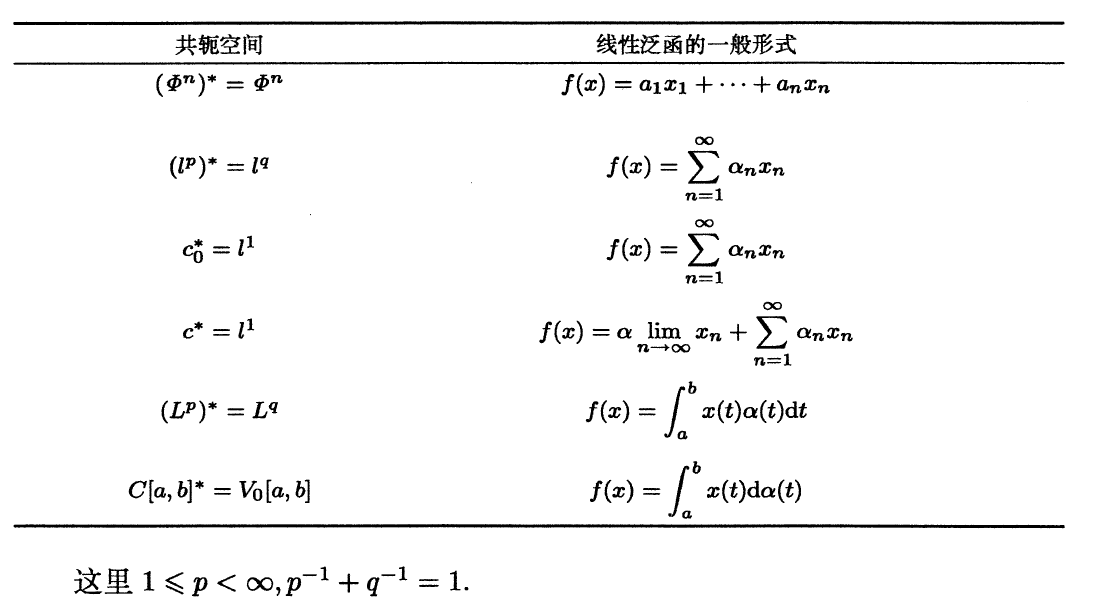
\includegraphics[width=0.8\linewidth]{11.png}
    \nonumber
    \label{fig:enter-label}
\end{figure}

\subsubsection{共轭的复合:共轭空间上泛函 \& 自然嵌入算子}
\begin{enumerate}
    \item 对于共轭空间$X^*$,我们可以定义一簇有界线性泛函$x^{**}:x^{**}(f)=f(x),\forall f \in X^*$ 由于$\lvert \lvert x^{**} \rvert \rvert=\sup_{\lvert \lvert f \rvert \rvert \leq 1}\lvert f(x) \rvert$ 根据前面$\text{Hahn-Banach}$定理的推论:$\lvert \lvert x^{**} \rvert \rvert=\lvert \lvert x \rvert \rvert$
    \item 这时我们转向考虑$X$与$X^{**}$之间的关系,于是我们定义了自然嵌入算子$J:Jx=x^{**}$ 其中$x^{**}:x^{**}(f)=f(x),\forall f \in X^*$就是我们上面考虑的那一组泛函。
    \begin{enumerate}
        \item $J$ 是$X$与$X^{**}$的一个线性子空间($\{ x^{**} \}$ 全体)的等距同构
        \item $\overline{J(X)}$ 是$X$的完备化空间 ($X^{**}$ 是$\text{Banach}$空间)
        \item 对于空间$X$一个的认识:既可以是$X$一个点,也可以是$X^{**}$一个点(作为$X^*$的泛函)
    \end{enumerate}
\end{enumerate}

\subsubsection{$w$收敛/有界/序列闭/序列紧/序列完备;$w^*$收敛}
\begin{enumerate}
    \item $w \text{-convergence} :\forall f \in X^* (x_{n},f)\to(x,f)$
    \item $w \text{-bounded} \ E: \forall f \in X^*,\exists M_{f}:(x,f)<M_{f},\forall x \in E$
    \item $w\text{-convergence} \underset{ \text{显然} }{\overset{ \text{存在凸组合} }{  \large{\rightleftharpoons} } } s\text{-convergence}$
    \item $w\text{-convergence} \overset{ \dim<\infty }{ \iff } s\text{-convergence} \overset{ \dim<\infty }{ \iff } \text{按坐标收敛}$
    \item $w\text{-bounded} { \iff } s\text{-bounded}$
    \item $x_{n} \overset{ w }{ \to } x  \iff   \{ x_{n} \} s\text{-bounded} \ \& \ \exists \ G \subset X^*:\overline{\mathrm{span}(G)}=X^*;\forall f \in G: f(x_{n}) \to f(x)$
    \item $A \ s\text{-closed} \overset{ \text{concavity} }{ \iff } A \ w\text{-series closed}  \qquad \text{(凸集分离定理)}$
    \item $w \text{-serial compact}: \text{任意点列存在}w\text{-收敛子列}$
    \item $w \text{-serial complete}: \text{任意}w\text{-Cauchy}\text{序列都是}w{-收敛序列}$
    \item $w^* \text{-convergence}: \forall x \in X:(x,f_{n} )\to(x,f)\qquad \text{(逐点收敛)}$
\end{enumerate}

\subsubsection{共轭算子}
给定$T:X\mapsto Y$ 定义$T^*:Y^* \mapsto X^*:(Tx,y^*)=(x,T^*y^*),\forall x\in X,y^* \in Y^*$ 为共轭算子。可以证明
它的存在是普遍的、唯一的、保范的,它是线性代数中转置矩阵的推广。

而对于共轭算子的共轭算子$T^{**}:X^{**} \mapsto Y^{**}$。它是$T$的保范线性延拓。
$$(y^*,A^{**}x)=(y^*,A^{**}x^{**})=(A^*y^*,x^{**})=(A^*y^*,x)=(y^*,Ax),\forall y\in Y^*,x \in X$$

\subsubsection{紧算子、有限秩算子}
\begin{enumerate}
    \item 顾名思义,紧算子就是将有界集映为相对紧集的线性算子;有限秩算子就是$\dim T(x)<\infty$的线性算子
    \item 基于第一章,我们可以得到:
    \begin{enumerate}
        \item 紧算子全体$C(X,Y)$是$B(X,Y)$的线性子空间;当$Y$是Banach空间时,$C(X,Y)$是闭子空间,从而也是Banach空间。
        \item 有界的有限秩算子是紧算子,因为有限维空间中,范数有界集等价于相对紧集。
    \end{enumerate}
    \item 与共轭算子联动可以得到:紧算子的共轭算子也是紧算子。
    \item 紧算子的强大之处:将弱收敛序列映射为强收敛
    \item 对于有Schauder基的Banach空间,紧算子可以表示为一列有限秩算子的极限。
\end{enumerate}
\subsection{习题}
% \begin{theorem}
% 1:
% \end{theorem}
% \begin{theorem}
% 2:
% \end{theorem}
% \begin{theorem}
% 3:
% \end{theorem}
\begin{theorem}
4:证明泛函序列 $f_n(x) = \int_{-\pi}^{\pi} x(t) e^{int} \, dt$ 在 $L^2[-\pi,\pi]$ 上弱收敛于 0。
\end{theorem}


\begin{theorem}
5:设 $X$ 是线性赋范空间,$X^{*}$ 是 $X$ 的共轭空间,$x_n, x \in X$,$f_n, f \in X^*$。若 $x_n \overset{w}{\rightarrow} x$,$f_n \overset{s}{\rightarrow} f$,则 $f_n(x_n) \rightarrow f(x)$。举例说明,当二者皆为弱收敛时结论不必成立。
\end{theorem}

\begin{proof}
因为$|f_n(x_n)-f(x)| \leq |f_n(x_n)-f_n(x)|+|f(x)-f_n(x)|\leq 2\varepsilon$,前者由于$x_n \to x$,后者因为$f_n \overset{w}{\rightarrow} f$。
\\
反例:设$X=c_0:X^*=l^1$,取$x_n=e_n$,则$x_n\overset{w}{\rightarrow}x:=0$;取$f_n=(1,1,1,\cdots 0 \cdots)\overset{w}{\rightarrow}f:=(1,1,1,\cdots 1 \cdots)$
。此时$f_n(x_n)=1,f(x)=0$,矛盾。
\end{proof}

\begin{theorem}
6:若$T \in B(X,Y),x_n,x \in X,x_n \overset{w}{\to} x$,则$Tx_n\overset{w}{\to} Tx$
\end{theorem}

\begin{proof}
$\forall g \in Y^*:(Tx,g)=(x,T^*g)$,由于$T^*g \in X^*,x_n \overset{w}{\rightarrow}x$。所以$(Tx_n,g) \to (Tx,g),\forall g \in Y^*$。
\end{proof}

\begin{theorem}
7:验证泛函序列$g_n(x)=\int_0^1 x(t)t^n \, dt$在$\mathscr{L}^\infty[0,1]$上$w^*$收敛于0
\end{theorem}

\begin{proof}
根据$H\ddot{o}lder$不等式可以直接得出。
\end{proof}

\begin{theorem}
8:$X$是Banach空间,则它的共轭空间$X^*$中的$w^*$有界集是范数有界集。
\end{theorem}

\begin{proof}
$w^*$有界集$E$:$\forall x \in X ,f \in E:f(x)<\infty\to E$是一族在第二刚集$X$上点点有界的有界线性泛函。
从而依据共鸣定理,$E$范数有界。
\end{proof}

\begin{theorem}
9:利用开映射定理证明:若 $X$ 是Banach空间,$J: X \rightarrow X^{**}$ 是自然嵌入算子,并且 $X$ 不是自反的,则 $J(X)$ 在 $X^{**}$ 中是第一纲集。
\end{theorem}

\begin{proof}
反证:如果$J(X)$是第二纲集,那么根据开映射定理,$J$是到上的,从而是自反的,矛盾。
\\
*开映射定理:Banach 空间 $X$ 到线性赋范空间 $Y$ 的有界线性算子 $T$,如果像集$R(T)$是第二纲集,则 $T$ 是开算子且满射;Banach 空间 $X$ 到Banach 空间 $Y$ 上的有界线性算子 $T$ 是开算子
\\
*逆算子定理:Banach 空间 $X$ 到线性赋范空间 $Y$ 的一一的有界线性算子 $T$,如果像集$R(T)$是第二纲集,则 $T^{-1}$ 是线性赋范空间 $Y$ 到 Banach 空间 $X$ 的有界线性算子,且 $Y$ 是 Banach 空间
\end{proof}

\begin{theorem}
10:证明弱下半连续泛函是下半连续的,每个范数都是弱下半连续的
\end{theorem}

\begin{proof}
弱下半连续泛函$f:\forall x, x_n \overset{w}{\rightarrow} x, \underset{n \to \infty}{\underline{\lim}} f(x_n)\geq f(x)$。
因为范数收敛强于若收敛,弱下半连续是下半连续的充分条件;同时,范数是连续的泛函,自然是弱下半连续泛函。
\end{proof}

\begin{theorem}
11:设 $\{x_n\}$ 是 $C[a,b]$ 中的有界序列,若 $\forall t \in [a,b]$,$x_n(t) \rightarrow x(t)$,则存在 $\{x_n\}$ 的凸组合的序列在 $[a,b]$ 上一致收敛于 $x$。
\end{theorem}

\begin{proof}
根据例3.2.4和定理3.2.5即可得出结论
\end{proof}

\begin{theorem}
12:设 $1 \leqslant p < \infty$,$\{x_n\}$ 是 $l^p$ 中的一列元素,则存在 $\{x_n\}$ 的线性组合的序列以范数收敛于 $x_0$ 当且仅当 $\forall f \in (l^p)^*$,$f(x_n) = 0$ 时,$f(x_0) = 0$。
\end{theorem}

\begin{proof}

\end{proof}

\begin{theorem}
13:证明空间$c_0$不是弱序列完备的空间。
\end{theorem}

\begin{proof}
举反例:考虑$x_n=(1,1,1,\cdots,1,0,0,\cdots)$,则$x_n$是弱柯西列,但$x_n \overset{w}{\rightarrow}(1,1,1,\cdots 1 \cdots)$ \\ $\notin c_0$。所以$c_0$不是弱序列完备的空间。
\end{proof}

\begin{theorem}
15:证明$l^2$的闭单位球面$S_p(l^2)$是范数闭集但不是弱序列闭集。
\end{theorem}

\begin{proof}
由范数的连续性可以得出$S_p(l^2)$是一个范数闭集;下面举反例证明$S_p(l^2)$不是弱序列闭集:
取$x_n=e_n$,则$e_n\overset{w}{\rightarrow}0 \notin S_p(l^2)$,极限定义在$S_p(l^2)$外了。
\end{proof}

\begin{theorem}
16:设有 $T: l^p \rightarrow l^q$ ($1 < p < \infty$),$T(x_1, x_2, \cdots) = (0, x_1, x_2, \cdots)$,试求 $T$ 的共轭算子 $T^*$。
\end{theorem}

\begin{proof}
记$l^p$上有界线性泛函的一般形式为$f(x)=\sum_{n=1}^\infty \alpha_n x_n$。以共轭算子定义:$\sum_{n=1}^\infty \alpha_{n+1} x_n=(Tx,f)=(x,T^*f)=\sum_{n=1}^\infty (T^*\alpha_n) x_n$
。所以$T^*\alpha_n=\alpha_{n+1}$。
\end{proof}

\begin{theorem}
18:设 $1 < p < \infty$,证明线性算子
$$T: l^p \rightarrow l^p, \quad (x_1, x_2, \cdots) \rightarrow (x_1, \frac{x_2}{2}, \frac{x_3}{3}, \cdots)$$
是紧算子。
\end{theorem}

\begin{proof}
考虑算子序列$T_n(x)=(x_1, \frac{x_2}{2}, \frac{x_3}{3}, \cdots, \frac{x_n}{n}, \cdots)$。则$T_n$是有界的有限秩算子,而且:
$||Tx-T_nx||=\left(\sum_{i=n}^\infty |\frac{x_i}{i}^p|\right)^{\frac{1}{p}}\to 0,\forall x\in X$,所以$T_n \to T$。
又因为$C(l^p,l^p)$是Banach空间,所以$T$是紧算子。
\end{proof}


\begin{theorem}
19:证明$T:C[0,1] \mapsto C[0,1],Tx(t)=\int_0^tx(\tau)\,d\tau$是紧算子,而$Sx(t)=tx(t)$不是紧算子
\end{theorem}

\begin{proof}
对于$T$,根据Arzela-Ascoli定理,可以证明$T(A:\text{C[0,1]中的有界集})$是紧集,从而$T$是紧算子。下面证明$T(A)$是等度连续的。
首先对于每一个$T(x)$,由积分的绝对连续性可知其一致连续。给定$\varepsilon>0$,存在$\delta:\forall Tx(t)\in A$,只要$|t_1-t_2|<delta$,就有
$|Tx(t_1)-T(x_t2)|<\varepsilon$,从而可以证明其等度连续。

对于$S$,
\end{proof}

\begin{theorem}
20:$X$是线性赋范空间,$Y$是Banach空间,$T \in B(X,Y)$。证明:若$T^*$是紧算子,那么$T$也是
\end{theorem}

\begin{proof}
如果$T^*$是紧算子,那么$T^{**}:X^{**} \mapsto Y^{**}$也是紧算子。同时,因为$Y \subset Y^{**}$是Banach空间,
$Y$是$Y^{**}$的闭子空间,所以$Y \subset Y^{**}$上的点列在$Y$上定义。考虑有界的点列$x_n^{**} \in X \subset X^{**}$,记自然嵌入算子$J$:
则$T^{**}(x_n^{**})=T^{**}J(x_n)=JT(x_n)=(T(x_n))^{**}$,所以$T(X_n) \in Y\subset Y^{**}$。根据$T^{**}$紧算子性质,
$T(X_n)$存在收敛子列,所以$T$是紧算子。
(这个题是定理3.3.5的逆命题,但是二者不等价,欲使逆命题成立需要加强$Y$是Banach空间)
\end{proof}

\begin{theorem}
21:设 $X$ 是Banach空间,$\dim X < \infty$. $T: X \rightarrow X$ 是紧算子,则 $T$ 是一一的就不可能是到上的。
\end{theorem}

\begin{proof}
反证:假设$T$是一一且到上的。那么根据逆算子定理:$T$是$X$与$X$之间的同构映射。所以$\dim(T(X))=\infty$,从而$T(A:\text{X中的有界集})$就不再是相对紧集,矛盾。
\end{proof}

\begin{theorem}
22:设 $X$ 是线性赋范空间,$T \in B(X)$,$T$ 紧并且 $T^2 = T$,则 $\dim T(X) < \infty$。
\end{theorem}

\begin{proof}
考虑$T|_{T(X)}$,则$T|_{T(X)} (x:=T(u))=TT(u)=T(u)=x$,所以$T|_{T(X)}$是恒等算子。又因为$T$是紧算子,
根据$T$连续性,$T|_{\overline{T(X)}}$是恒等算子;从而$\overline{T(X)}$中的有界集就是相对紧集,$\dim T(X) < \infty$。
\end{proof}

(上面两个题用到了一个第一章的重要结论:有限维空间的等价条件是有界集是相对紧的)

\section{Hilbert空间的几何学}
\subsection{知识点速览}
下面$H$若无明确指代,则指内积空间
\subsubsection{正交集、正交基}
\begin{enumerate}
    \item 对于$H$中的标准正交集$\{e_n\}$:以下是必要条件
    \begin{enumerate}
        \item $\forall x\in X$:Bessel不等式成立
        \item 数集$\{(x,e_n)\}$至多有可数多个非零元,不然就无限大了
        \item $(x,e_n)\to 0 \forall x\in X \iff e_n\overset{w}{\to}0$(剧透一下Riesz表示定理)
    \end{enumerate}
    \item 对于$H$中的标准正交集$\{e_n\}$:以下命题等价
    \begin{enumerate}
        \item $x\in \overline{\text{span}}(e_n)$
        \item $x=\sum_{n=1}^\infty  (x,e_n)e_n$,即可以进行Fourier展开
        \item $\forall x\in \overline{\text{span}}(e_n)$,Parseval等式成立,即Bessel不等式取等
    \end{enumerate}
    \item Riesz-Fischer:对于Hilbert空间的标准正交集$\{e_n\}$,对于任意$\alpha\in l^2$:存在 \\ $x\in \overline{\text{span}}(e_n):x=\sum_{n=1}^\infty \alpha_n e_n,\alpha_n=(x_n,e_n)$
    \item 对于Hilbert空间$H$中的标准正交集$E$:以下命题等价
    \begin{enumerate}
        \item $E$是正交基
        \item $\overline{\text{span}}(E)=H$
        \item $\forall x\in H$可以进行Fourier展开
        \item $E$是完备正交集($\forall x\in H$,Parseval等式成立)
        \item $\forall x,y\in H:(x,y)=\sum_{n=1}^\infty (x,e_n)\overline{(y,e_n)}$
        \item $E$是完全正交集($x \perp E \to x=0$)
    \end{enumerate}
\end{enumerate}

\subsubsection{Hilbert空间的结构}
如果Hilbert空间$H$的正交基$\{e_n\}$是可数的,那么它是可分的;如果$\{e_n\}$个数有限,则Hilbert空间$H$等距同构于$\Phi^n$;
如果$\{e_n\}$个数可数无限,则Hilbert空间$H$等距同构于$l^2$。
\subsubsection{内积空间中的点在线性子空间/凸子集上的投影}
\begin{enumerate}
    \item 投影的定义基于正交分解:给定线性子空间$E$,点$x$可以做如下分解:$x=y+z,y\in E,z\perp E$。我们称$y=P_E x$为$x$关于$E$的正交投影。
    \item 投影点$y$就是子空间$E$关于点$x$的最佳逼近元。
    \item 如果$E$是闭子空间,$H$是Hilbert空间,则$\forall x\in H$,$P_Ex$(最佳逼近元)存在且唯一。
\end{enumerate}
\subsubsection{Hilbert空间中的投影算子}
投影算子$P_E:H(\text{Hilbert})\mapsto E(\text{closed  linear subspace})$
\begin{enumerate}
    \item $P_E$是线性算子
    \item $||P_E||=1\iff E\neq\varnothing$
    \item $E=R(P_E)=N(I-P_E),N(P)=R(I-P_E)$
\end{enumerate}

对于Hilbert空间$H$的子空间$E$,我们可以定义$E^{\perp}$为正交于$E$的元素全体。
\begin{enumerate}
    \item $E^{\perp}$是$H$的闭线性子空间
    \item 如果$E$是闭集,$E^{\perp\perp}=E$;$H=E \oplus E^{\perp}$,此时称$E^{\perp}$是$E$的正交补。
\end{enumerate}

投影算子之间的关系
\begin{enumerate}
    \item 定义$P_E \leq P_F \iff E \subset F$,它等价于以下条件:
    \begin{enumerate}
        \item $||P_Ex||\leq||P_Fx||,\forall x \in H$
        \item $P_EP_F=P_FP_E=P_E$
        \item $P_F-P_E$是投影算子
    \end{enumerate} 
    \item 如果$E\perp F$,则以下条件等价:
    \begin{enumerate}
        \item $R(P_E)\perp R(P_F)$
        \item $P_EP_F=0$
        \item $P_F+P_E$是投影算子
    \end{enumerate}
    \item 一列点点收敛的投影算子的极限是投影算子
    \item 两两正交的投影算子的和点点收敛于一个投影算子
    \item 一列递升的投影算子$P_{E_n}$点点收敛于一个投影算子$P_E:E=\overline{\bigcup_{n=1}^\infty E_n}$
\end{enumerate}
\subsubsection{Hilbert空间中的伴随算子和自伴算子}
\begin{enumerate}
    \item 伴随算子:$(Tx,y)=(x,T^*y)$,此处是内积,而非泛函作用;作为线性代数中共轭转置矩阵的推广。
    \item 自伴算子:$T^*=T:(Tx,y)=(x,Ty)$
    \item 投影算子的充要条件:幂等的自伴算子;幂等算子且$N(P)\perp R(P)$;复空间内:$(Px,x)=||Px||^2,\forall x\in H$
    \item $N(T)=R(T^*)^{\perp};N(T^*)=R(T)^{\perp};\overline{R(T)}=N(T^*)^{\perp};\overline{R(T^*)}=N(T)^{\perp}$
\end{enumerate}
\subsubsection{Hilbert空间$H$的共轭空间:Riesz表示定理}
$\forall f\in H^*,\exists y\in H:f(x)=(x,y),||f||=||y||$
\begin{enumerate}
    \item 从集合论来看,$H^*=H$,从而$H$是自反空间
    \item 为了保证泛函关于$x$的线性,只能将$y$放在后面。
    \item 记$T:H^*\mapsto H:T(f)=y$,则$T$是共轭线性的:\\ $T(af_1+bf_2)(x)=af_1(x)+bf_2(x)=a(x,y_1)+b(x,y_2)=(x,\bar{a}y_1+\bar{b}y_2)$
    \item $(Tf,Tg)=\overline{(f,g)}=(g,f)$
\end{enumerate}
\subsubsection{一·五线性泛函(广义内积)的表现}
对于定义在$H(\text{Hilbert})\times H(\text{Hilbert})\mapsto \Phi$的映射$\phi$:
\begin{enumerate}
    \item 所谓的一·五线性就是满足以下条件:
    \begin{enumerate}
        \item $\phi(ax+by,z)=a\phi(x,z)+b\phi(y,z)$
        \item $\phi(z,ax+by)=\bar{a}\phi(z,x)+\bar{b}\phi(z,y)$    
    \end{enumerate}
    \item 称$\phi$是对称的$\iff \, \phi(x,y)=\overline{\phi(y,x)}$
    \item 称$\phi$是有界的$\iff \, |\phi(x,y)|\leq C||x|| \, ||y||$,此时定义算子范数$||\phi||=\underset{||x||,||y||\leq 1}{\sup}|\phi(x,y)|$
    \item 在Hilbert空间$H$中,$\phi$是有界的一·五线性泛函 $\iff$ 存在$T\in T(H):\phi(x,y)=(Tx,y),||\phi||=||T||$
    \item 在Hilbert空间$H$中,$A\in B(H)$是自伴算子 $\iff$ 一·五线性泛函$\phi(x,y)=(Ax,y)$是对称的;若$\Phi=\mathbb{C}$,则还等价于$\phi(x,x)=(Ax,x)\in \mathbb{R}$
\end{enumerate}


\subsubsection{Hilbert空间上几个特殊的算子:酉算子、正规算子}
\begin{enumerate}
    \item 定义酉算子:$TT^*=T^*T=I:\text{单位算子}\iff (Tx,Ty)=(x,y)\,\forall x,y \in H$
    \item 定义正规算子:$TT^*=T^*T\iff ||Tx||=||T^*x|| \forall x\in H$
    \item $T$是正规算子$\iff T=T_1+iT_2,T_1T_2=T_2T_2;T_1,T_2\text{是自伴算子}$
    \item 正规算子的(依范数收敛的)极限也是正规算子
\end{enumerate}

\subsection{习题(偶数题)}

\begin{theorem}
2:设$H$是内积空间,$x,y_i \in H(i \geq 1)$,证明:

(1) $x \perp \overline{span}\{ y_i:i\geq 1 \} \iff x \perp y_i(i \geq 1)$

(2) $x \perp \overline{co}\{ y_i:i\geq 1 \} \iff x \perp y_i(i \geq 1)$
\end{theorem}


\begin{theorem}
4:设$H$是Hilbert空间,$\{ x_n \}$是规范正交集。证明以下三条等价:

(1) $\sum_{n=1}^\infty x_n$收敛  (2) $\forall y\in H,\sum_{n=1}^\infty (x_n,y)$收敛  (3) $\sum_{n=1}^\infty ||x_n||^2$收敛
\end{theorem}

\begin{proof}
$(1)\Rightarrow (2)$:设$x:=\sum_{n=1}^\infty x_n$,则对于$\forall y \in H:\sum_{n=1}^N (x_n,y) =(\sum_{n=1}^N x_n,y)\to  (\sum_{n=1}^\infty x_n,y)=(x,y)$
\\
$(2)\Rightarrow (3)$:由$(2)$知,$\forall y\in H,(x_n,y)\to 0$,所以$x_n \to 0$,$||x_n||^2\to 0$。所以$\sum_{n=1}^N ||x_n||^2$收敛
\\
$(3)\Rightarrow (1)$:由$(3)$知,$\{\sum_{n=1}^N x_n\}$是柯西列,由于$H$是Hilbert空间,$\{\sum_{n=1}^N x_n\}$收敛
\end{proof}

% \begin{theorem}
% 6:
% \end{theorem}

% \begin{theorem}
% 8:
% \end{theorem}

% \begin{theorem}
% 10:
% \end{theorem}

\begin{theorem}
12:设$f\in\mathscr{L}^2[a,b]$(实空间),若$\int_a^bf(t)t^n\,dt=0,n\geq0$,则$f(t)=0,\text{a.e.}$
\end{theorem}

\begin{proof}
由题目知$f\perp \{ \text{实多项式全体}\}$,而实多项式全体在$C[a,b]$上面稠密,$C[a,b]$在$\mathscr{L}^2[a,b]$上面稠密.
所以$f\perp y,\forall y \in \mathscr{L}^2[a,b]$。从而$f=0,\text{a.e.}$。($\mathscr{L}^2[a,b]$将几乎处处相等的两个函数视为同一个点)
\end{proof}

\begin{theorem}
14:举例说明当$H$不是完备内积空间时,定理4.1.6的(4)(6)不等价
\end{theorem}


\begin{theorem}
16:若$E \subset H$是线性子空间,且$\forall x\in X$,$x$在$E$上的投影存在,则$E$是闭的
\end{theorem}

\begin{proof}
设有$E$中点列$x_n \to x_0$,下证$x_0 \in E$。记$x_0$关于$E$的正交分解为$x_0=y+z,y\in E,z\perp E$,
从而$z \perp x_n$。$0=\lim_{n\to\infty}(x_n,z)=(x_0,z)=||z||=0$,所以$z=0$,从而$x_0 \in E$
\end{proof}

\begin{theorem}
18:若$P_1,P_2$是投影算子,则$P_1P_2$是投影算子$\iff \ P_1P_2=P_2P_1$
\end{theorem}

\begin{proof}
只需验证$P_1P_2$是幂等、自伴算子
\end{proof}

*下面的$H$均为复Hilbert空间。

\begin{theorem}
20:设$P_n$是$H$上的投影算子序列,并且$P_n \leq P_{n+1}$,证明存在投影算子$P$,使得$P_n\to P$是逐点收敛
\end{theorem}

\begin{proof}
法1:记$E_n$为$P_n$对应的闭线性子空间:$P_n\leq P_{n+1}\iff E_n \subset E_{n+1}$,此时根据定理4.2.7(2):
取$P=P_E,E=\overline{\bigcup_{n=1}^\infty E_n}$,则$P_n \to P$是逐点收敛。
\\
法2:$\forall x \in H$,$||P_n(x)||$是单调递升有上界(Bessel不等式)的数列,所以存在极限,记为$||Px||$。
所以$P_n \to P$是逐点收敛;依据引理4.2.1:$P$是投影算子。
\end{proof}

\begin{theorem}
22:设 $E \subset H$ 是闭凸集,$x \in H$,为了 $x_0$ 是 $x$ 关于 $E$ 的最佳逼近元,必须并且只须
\[
\text{Re}(x - x_0, y - x_0) \leq 0, \quad \forall y \in E.
\]
\end{theorem}


\begin{theorem}
24:设$A \in B(H)$,证明$A+A*=0 \iff \text{Re}(Ax,x)=0,\forall x \in H$
\end{theorem}

\begin{proof}
$\Rightarrow$:$A+A*=0 \Rightarrow (Ax,x)=-(x,Ax)=-\overline{(Ax,x)},\forall x \in H$,从而: \\ 
$\text{Re}(Ax,x)=0,\forall x \in H$
\\
$\Leftarrow$:$\forall x\in H:((A+A^*)x,x)=(Ax,x)+(x,Ax)=2\text{Re}(Ax,x)=0$,从而 \\ $A+A^*=0$
\end{proof}

\begin{theorem}
26:证明$T:\mathscr{L}^2[a,b] \mapsto \mathscr{L}^2[a,b],Tx(t)=tx(t)$是自伴算子
\end{theorem}
\begin{proof}
直接按照定义验证即可
\end{proof}

\begin{theorem}
28:设 $\{e_n, n \geq 1\}$ 是 $H$ 中的规范正交集,$\lambda_n \in \Phi$,定义 $T: H \rightarrow H$,$T(x) = \sum_{n=1}^{\infty} \lambda_n(x, e_n)e_n$。证明若 $\lambda_n$ 是有界数列,则 $T \in B(H)$,$T$ 是自伴算子当且仅当 $\lambda_n$ 是实数。
\end{theorem}

\begin{proof}
有界算子的证明依据Bessel不等式即可。
\\ 
至于自伴算子的证明:\\ 
$(x,Ty)=(x,\sum_{n=1}^{\infty} \lambda_n(y,e_n)e_n)=\sum_{n=1}^{\infty} \overline{\lambda_n(y,e_n)}(x,e_n)=\sum_{n=1}^{\infty} \overline{\lambda_n}(e_n,y)(x,e_n)$
\\
$(Tx,y)=(\sum_{n=1}^{\infty} \lambda_n(x,e_n)e_n,y)=\sum_{n=1}^{\infty} {\lambda_n}(x,e_n)(e_n,y)$
\\ 所以二者相等当且仅当$\lambda=\overline{\lambda}\iff\lambda \in \mathbb{R}$
\end{proof}

\begin{theorem}
30:证明$T:\mathscr{L}^2[0,\infty) \mapsto \mathscr{L}^2[0,\infty),Tx(t)=x(t+a)$是酉算子
\end{theorem}
\begin{proof}
先将伴随算子按定义求出来,然后按定义验证$T$是酉算子即可
\end{proof}

\begin{theorem}
32:设$T$是$H$上面的紧算子,$\{e_n \}$是规范正交集,则$T{e_n} \to 0$ (用弱收敛证明)
\end{theorem}

\begin{proof}
由Riesz表示定理$\forall f \in H^*:\exists y\in H:f(x)=(x,y)$;由第四题:$\forall y\in H:(e_n,y)\to 0:e_n \overset{w}{\to} 0$
又因为$T$是紧算子,所以$T(e_n) \to 0$。(定理3.3.6:紧算子将若收敛点列映为强收敛点列)
\end{proof}

\begin{theorem}
34:设$U$是酉算子,则当$T$分别是投影算子、自伴算子、酉算子、正规算子时,$U^{-1}TU$也是
\end{theorem}
\begin{proof}
按定义逐个验证即可
\end{proof}
\end{document}
